\section{KC3DRES: The Resistor Toolbox}
The module \textbf{kc3dres} represents parametric models of resistors. 

\subsection{kc3dres:Resistor}
The class \textbf{Resistor} represents a thru-hole cylindrical resistor such as
the typical color-coded Carbon Composite Resistor or Metal Film Resistor. The
resistor model itself is generated by a simple command, in the example below it is
\verb#R.create(P, "11X55X66X22XXGG", "resistordemo")#, however the model takes
about 28 parameters which need to be set up beforehand.  The parameters are all
stored in the structure \textbf{kc3dres.RParams} and are as follows:

\begin{itemize}
\item\textbf{scale}: scale factor to apply to final result
\item\textbf{shift}: shift along X-axis to center reference point (usually 1/2 pitch)
\item\textbf{L}: length of resistor body
\item\textbf{D}: diameter of resistor body
\item\textbf{d}: diameter of wire
\item\textbf{p}: lead pitch
\item\textbf{wl}: wire length below top of PCB
\item\textbf{horiz}: True for horizontal orientation
\item\textbf{endshape}: resistor end style, `C'ap, `R'ound, or `B'ulge (default)
\item\textbf{bcap}: True if a Bulge style body also has metallic end caps
\item\textbf{wsides}: number of vertices in a wire cross-section
\item\textbf{bsides}: number of segments in a right angle bend
\item\textbf{rsides}: number of vertices in the resistor body cross-section
\item\textbf{pwrsuf}: optional suffix to indicate power rating, ex: ``0W25''
\item\textbf{spcsuf}: optional suffix to indicate lead spacing and orientation, ex: ``0I40H''
\item\textbf{colors}: colors mapped to the color code, body color, wire color
\end{itemize}

The \textbf{colors} parameters cannot be accessed directly; use the helper function
\textbf{setRColors(index, params, colorfile)} to set the colors. The indices are
0 to 9 to represent the code for the digits 0 to 9, 10 for gold, 11 for silver,
12 for the body color, and 13 for the wire color.

To create the 3D model, set up the parameters and then invoke
\textbf{create(params, code\_string, base\_name)} where params is the
set of parameters previously set up, code\_string is a string representing
the colored bands and gaps, and base\_name is the base filename; the
routine will add the endstyle code, power suffix, lead space suffix, and the
suffix ``.wrl'' to produce the full file name. The recommended format for the
base name is \textbf{[Part Series]\_[Value]\_[Tolerance][T coeff]}, for example
``CCR\_11R\_J-'' is a generic carbon composite (part series) with $11\Omega$
resistance, tolerance class J, with no specified temperature coefficient.
The code string is a series of characters from the set 0..9, G, S, X and
each character represent a band on the resistor. Repeat characters as
necessary to obtain the required band widths and spacings; you may even
add a temperature coefficient band. In the example below, the string
``11X55X66X22XXGGG'' represents an imaginary 15.6K resistor with $5\%$
tolerance; the tolerance band is 1.5 times the width of a value band.
As an example of the flexibility of this coding system, you can specify
a $0\Omega$ link with the code ``XXX0XXX''.

A wide variety of resistors (Series E96 + E24 for 0.5W 1\% MFR, Series E48
for 0.5W 2\% MFR, Series E24 for 0.25W 5\% CCR) have been rendered in
horizontal orientation with 0.4 inch lead spacing and in vertical
orientation with 0.2 inch lead spacing, so this module is most useful
for generating models which are not already available. The necessary
scripts and modules also take up much less storage space than the
pre-generated models so in the future the pre-generated models may
be discontinued and models may be generated via script as needed.

\begin{verbatim}
import kc3d
import kc3dres
from kc3d import *
from kc3dres import *

R = Resistor()
P = RParams()

# load the colors for the resistor codes, body, and wires
setRColors(0, P, "../colors/rcc_blk_g.mat")
setRColors(1, P, "../colors/rcc_brn_g.mat")
setRColors(2, P, "../colors/rcc_red_g.mat")
setRColors(3, P, "../colors/rcc_org_g.mat")
setRColors(4, P, "../colors/rcc_yel_g.mat")
setRColors(5, P, "../colors/rcc_grn_g.mat")
setRColors(6, P, "../colors/rcc_blu_g.mat")
setRColors(7, P, "../colors/rcc_pur_g.mat")
setRColors(8, P, "../colors/rcc_gry_g.mat")
setRColors(9, P, "../colors/rcc_wht_g.mat")
setRColors(10, P, "../colors/rcc_gld_g.mat")
setRColors(11, P, "../colors/rcc_slv_g.mat")
setRColors(12, P, "../colors/rbc_blu_g.mat")
setRColors(13, P, "../colors/tin.mat")

# set the resistor parameters
P.scale = 0.3937
P.shift = -2.54
P.L = 6.3
P.D = 2.3
P.d = 0.6
P.wl = 2.0
P.p = 5.08
P.horiz = False
P.endshape = 'B'
P.bcap = True
P.wsides = 16
P.bsides = 5
P.rsides = 48
P.pwrsuf = "0W50"
P.spcsuf = "0I20"

R.create(P, "11X55X66X22XXGGG", "resistordemo")
\end{verbatim}


\begin{figure}
\label{fig:k3dres-horiz}
\centering
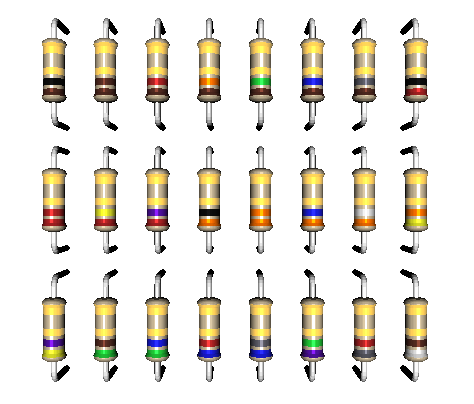
\includegraphics[width = 0.5\textwidth]{img/k3dres-horiz.png}
\caption{Sample of first decade of horizontal carbon composite resistors,
0.4 inch pitch, series E24, 0.25W, 5\% tolerance.}
\end{figure}

\begin{figure}
\label{fig:k3dres-vert}
\centering
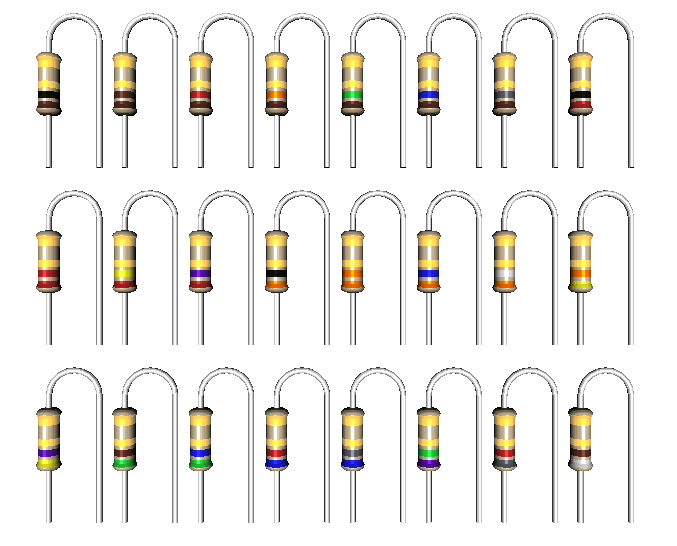
\includegraphics[width = 0.5\textwidth]{img/k3dres-vertical.png}
\caption{Sample of first decade of vertical carbon composite resistors,
0.2 inch pitch, series E24, 0.25W, 5\% tolerance.}
\end{figure}
